\documentclass[../main.tex]{subfiles}
\begin{document}
\section{Introduction}

Denmark, like many developed countries, has undergone and is still undergoing a significant demographic transition where increasing longevity and low fertility are leading to an aging population, see figure \ref{fig:Old-age-dep_intro}. In recent years, this demographic transition has caused attention as a possible force behind the decline in the natural rate of interest (NRI) since the mid-1980s. Our motivation for this paper is to investigate the demographic transition's impact on the NRI in order to explain declining interest rates and suggest pension system reforms based on proposed changes by the Danish government to counteract similar low-interest rate environments in the future. 

The NRI was first defined by \textcite{wicksell1936interest} as the interest rate that characterises an economy in equilibrium with full employment and constant inflation abstracting from cyclical tendencies.\footnote{In other literature, the NRI is also defined as the equilibrium real interest rate or natural real rate. However, these different definitions are equivalent. As the NRI cannot be measured directly, we target the values of real interest rate around 2000-2007 in our simulations, a time where the Danish economy was closest to equilibrium in recent times.} It can then be interpreted as a benchmark for conducting monetary policy. In low interest rate environments, there are limited possibilities for conventional monetary policy as an instrument to stimulate economic activity and generate growth, which will make it difficult to break out of periods with low growth and low interest rates - or more popularly denoted secular stagnation as coined by \textcite{summers2014us}. 

The dynamics between demographics and the NRI are closely related to saving behaviour. Most importantly, higher life expectancy puts downward pressure on the NRI as households increase their savings in anticipation of a longer retirement period. This will result in a decreased marginal product on capital which will imply a lower interest rate. Secondly, a lower population growth (or shrinking workforce) leads to a higher capital-labour ratio which also leads to a declined marginal product on capital and puts further downward pressure on the natural interest rate. 
    \begin{figure}[H]
        \centering
        \begin{minipage}{0.45\textwidth}
            \centering
            \caption{Real interest rate (\%)}
            \label{fig:Real_interest_rate_DK }
            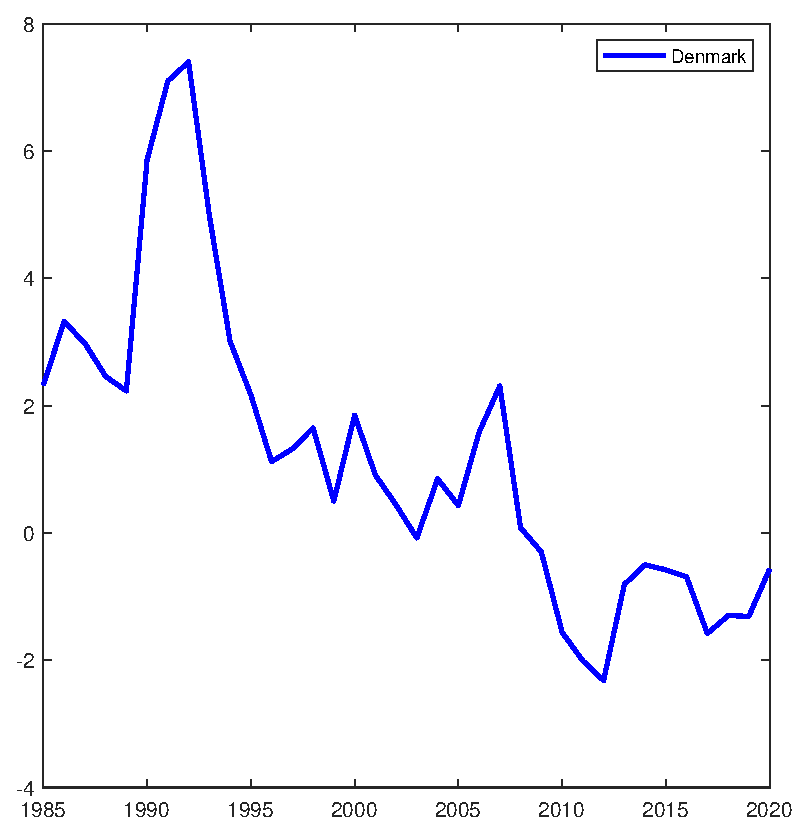
\includegraphics[width=0.95\textwidth]{Figures/Figure_0.eps} % first figure itself
        \end{minipage}
        \begin{minipage}{0.45\textwidth}
            \centering
            \caption{Old-age dependency ratio (\%)}
            \label{fig:Old-age-dep_intro}
            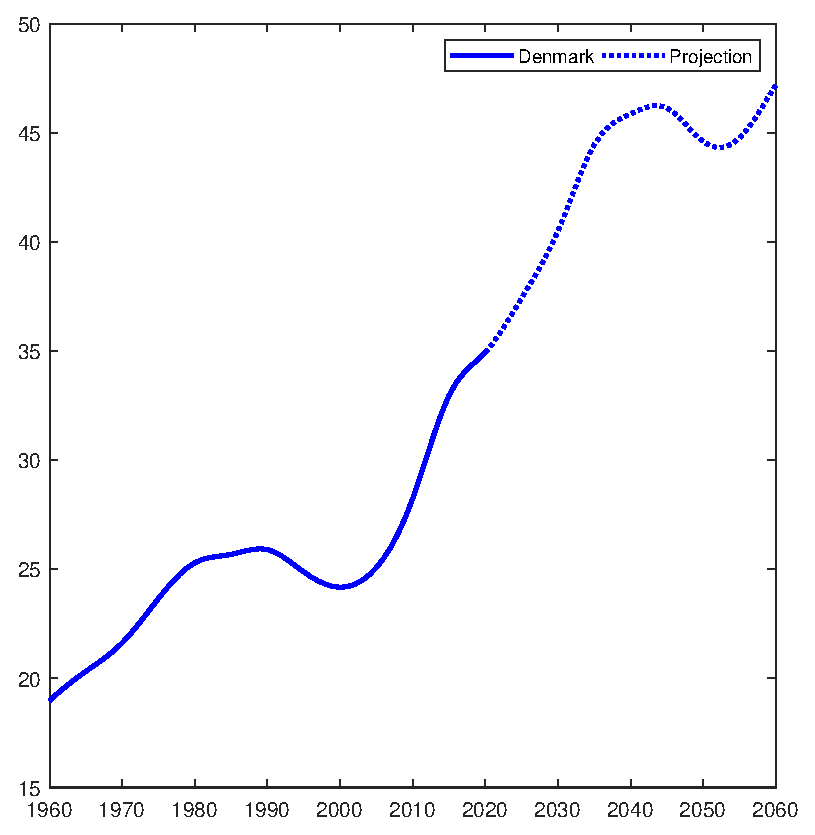
\includegraphics[width=0.95\textwidth]{Figures/Figure_1B.eps} % second figure itself
        \end{minipage}
        \begin{fignote}
                Data for real interest rate is Nationalbanken's DISKONTO minus inflation (consumer price index), table DNRENTA and PRIS9 from Statistikbanken respectively. Demographic data is from UN World Population Prospects 2019 (medium fertility variant). The old-age dependency ratio is defined as the ratio between the number of people aged 65 and above relative to the number of people aged 20-64.
                \end{fignote}
    \end{figure}
According to our findings, the NRI has fallen by 1.8 percentage points from 1985 to 2020, where demographics account for approximately half of that decline. We find that a decreasing mortality risk (higher lifetime expectancy) affects the NRI by -0.6 percentage points and low fertility by another -0.2 percentage points in this period. The rest of the decline is mainly due to sluggish TFP growth in the world.

Furthermore, aging population leads to the governmental challenge of ensuring public finance sustainability. In this regard, it is commonly known that the Danish government has suggested to increase the retirement age and/or decrease pension benefits. In section \ref{sec:policy_implications} we find that lower pension benefits will put a further downwards pressure on the NRI as workers increase their savings to finance consumption during retirement period. On the contrary, a higher retirement age puts upwards pressure on the NRI because workers save less in anticipation of a shorter retirement period. A combined adjustment has a net positive effect on the NRI implying that the effect of an increasing age dominates that of decreasing replacement rate.

There are several international studies investigating how the demographic transition has affected the NRI. We use the model setup by \textcite{bielecki2020demographics} that allows us to incorporate detailed registry life-cycle microdata combined with demographic data from the UN. Unlike \textcite{gagnon2021understanding} and \textcite{carvalho2016demographics} who use similar life-cycle models to estimate the NRI in the US and Euro-area respectively, we model a small open economy to capture the effect of cross-border capital flows and its effect on the domestic NRI. \textcite{gagnon2021understanding} finds that demographics is by and large the sole culprit of the decline in the NRI by 1.25 percentage points since 1980. \textcite{carvalho2016demographics} finds that for a representative developed economy, demographics account for about half of the decline in the NRI by 1.5 percentage points between 1990 and 2014. \textcite{eggertsson2019model} also implied a quantitative life-cycle model and find that demographic changes are the main forces behind secular stagnation in the US. \textcite{pedersen2015danish} finds that the Danish NRI is close to 0, possibly negative, and on a long-term negative trend.  

By applying an open economy OLG framework on Denmark with detailed demographic data and by taking suggested changes in the pension system into account, we consider this paper as a relevant expansion to the literature on the relationship between the demographic transition and the NRI in Denmark.


\end{document}